\section{模型评估和分析}

\subsection{数据集}

我们在给定的训练集和测试集上进行实验,其中训练集包含菜品ID、原料和烹饪风格(即菜系类别),测试集仅包含菜品ID和原料。菜品ID是唯一的数字序列,而原料由多个词组组成,每个词组中包含一个或多个小写英文单词。烹饪风格是模型需要预测的标签,由一个小写英文单词表示。我们将数据集的统计信息整理在表~\ref{tab:dataset}~中,表~\ref{tab:labels}~列出了数据集中的所有20种菜系类别。

\begin{table}[htbp]
    \centering
    \begin{tabular}{ccccccc}
        \toprule
         & 样本数 & 最大原料个数 & 最大单词个数 & 类别数 \\
        \midrule
        训练集 & 31819 & 65 & 136 & 20 \\
        测试集 & 7955 & 38 & 73 & - \\
        \bottomrule
    \end{tabular}
    \caption{数据集统计信息}
    \label{tab:dataset}
\end{table}

\begin{table}[htbp]
    \centering
    \resizebox{\textwidth}{!}{
    \begin{tabular}{cc|cc|cc|cc}
        \toprule
        brazilian & 巴西菜 & french & 法国菜 & jamaican & 牙买加菜 & russian & 俄国菜 \\
        british & 英国菜 & greek & 希腊菜 & japanese & 日本菜 & southern\_us & 美国南部菜 \\
        cajun\_creole & 克里奥尔菜 & indian & 印度菜 & korean & 韩国菜 & spanish & 西班牙菜 \\
        chinese & 中国菜 & irish & 爱尔兰菜 & mexican & 墨西哥菜 & thai & 泰国菜 \\
        filipino & 菲律宾菜 & italian & 意大利菜 & moroccan & 摩洛哥菜 & vietnamese & 越南菜 \\
        \bottomrule
    \end{tabular}%
    }
    \caption{全部菜系类别}
    \label{tab:labels}
\end{table}

\subsection{实现细节}

我们将菜品中所有原料对应的英文词组以空格分词,再将所有分词后的词语序列按顺序拼接为一个句子(严格地说,这里的句子不存在语法结构,仅由连续的单词构成),将其作为TextCNN模型的输入。在实验中,我们采用300维的GloVe预训练词向量\cite{pennington2014glove}作为词向量嵌入表征。我们还随机初始化了10维的位置编码,将其拼接在词向量后面构成单词的表征。对于没有出现在预训练词向量词表中的单词,我们使用均匀分布$U(-0.25,0.25)$对词向量进行随机初始化。在训练中,我们只更新位置编码,冻结GloVe预训练词向量。TextCNN的卷积窗口采用$\{3,4,5\}$三种大小,每种大小的卷积核各256个。我们使用Adam优化器\cite{kingma2014adam}训练模型,其中学习率设置为$10^{-4}$,权重衰减系数$\lambda=10^{-4}$。在训练中,我们使用余弦退火算法\cite{loshchilov2017sgdr}逐步减小学习率。我们选取训练集中的5\%样本作为验证集,在剩余的95\%样本上训练200轮,批处理大小为32,取验证集上准确率最高的一轮作为最优模型。由于离散的词语序列输入无法直接进行表征混合,因此我们选取池化后的句子表征和菜系类别标签进行混合,表征混合方法的超参数依照原文\cite{zhang2018mixup}设为$\alpha=1$。

\subsection{超参数调优}

我们使用K折交叉验证方法进行超参数的调优。具体地说,我们首先将训练集随机切分为20个互不相交的大小相同的子集,然后利用其中19个子集的样本训练模型,利用剩余的1个子集测试模型,并将该过程类似地重复20次,最后取平均测试结果最好的模型超参数作为最优超参数。

\subsection{结果对比}

经过模型训练和超参数调优,我们将TextCNN模型和其他方法进行对比,如表~\ref{tab:results}~中所示。评测指标采用准确率,即预测正确的样本占全部样本的比例。我们可以看到使用了数据增广方法的TextCNN模型取得了优于SVM方法和BERT模型的表现,并且深度集成后的TextCNN模型进一步提高了测试集上的准确率,最终在比赛工作站取得了第2名的成绩,如图~\ref{fig:rank}~所示。

\begin{table}[htbp]
    \centering
    \begin{tabular}{lc}
        \toprule
        \multicolumn{1}{c}{模型} & 准确率 \\
        \midrule
        SVM & 81.00$\pm$0.05 \\
        BERT & 81.18$\pm$0.12 \\
        TextCNN & 81.44$\pm$0.08 \\
        TextCNN(10$\times$) & {\bf 82.01}$\pm${\bf 0.06} \\
        \bottomrule
    \end{tabular}
    \caption{模型表现对比}
    \label{tab:results}
\end{table}

\begin{figure}[htbp]
    \centering
    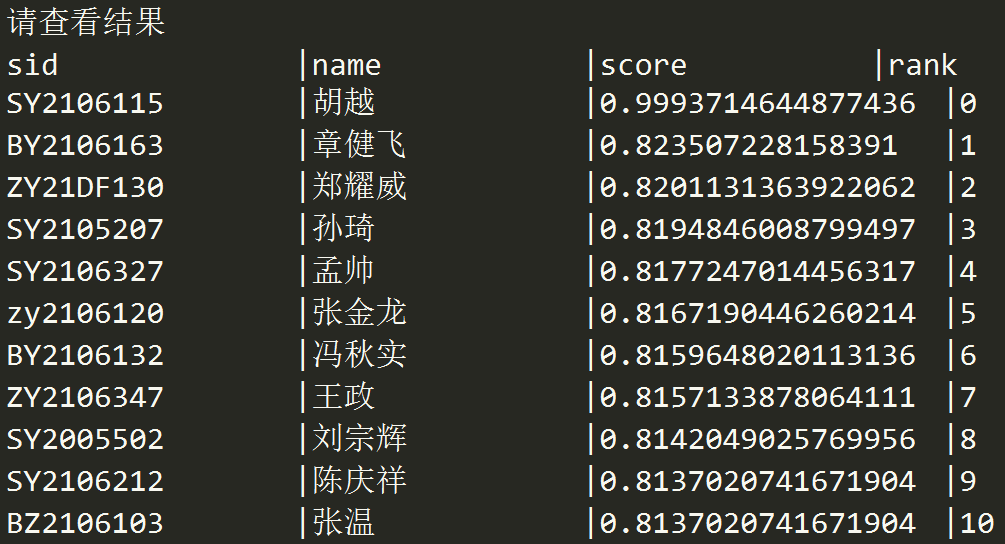
\includegraphics[width=.6\textwidth]{figs/rank.png}
    \caption{比赛工作站排名截图}
    \label{fig:rank}
\end{figure}


\subsection{消融实验}

为了验证模型设计中使用的多种方法与最终结果的关系,我们在数据集上进行了消融实验,实验结果呈现在表~\ref{tab:ablation}~中。根据实验结果,我们可以看到使用预训练词向量可以提供丰富的语义信息,提升了4\%左右的测试准确率。而数据增广方法缓解了标注数据匮乏的问题,带来了2\%左右的准确率提升。表征混合方法对模型施加了正则约束,在测试集上提升了1\%左右的准确率。深度集成方法进一步带来0.5\%左右的准确率提升。

\begin{table}[htbp]
    \centering
    \begin{tabular}{lc}
        \toprule
        \multicolumn{1}{c}{模型} & 准确率 \\
        \midrule
        TextCNN(10$\times$) & 82.01$\pm$0.06 \\
        TextCNN & 81.44$\pm$0.08 \\
        $\qquad$---表征混合方法 & 80.45$\pm$0.21 \\
        $\qquad$---数据增广 & 78.21$\pm$0.22 \\
        $\qquad$---预训练词向量 & 74.62$\pm$0.13 \\
        \bottomrule
    \end{tabular}
    \caption{消融实验结果}
    \label{tab:ablation}
\end{table}

\subsection{可视化分析}

为了进一步分析模型的工作原理,我们将TextCNN池化层的输出特征,也是Softmax层的输入特征进行可视化分析。我们在数据集中随机选取了200个样本,使用t-SNE\cite{van2008visualizing}降维方法,在图~\ref{fig:visualization}~中绘制出了2维平面上特征的分布。我们可以看到神经网络模型的高层特征具有良好的聚类特征,验证了模型具备较为可靠的分类效果。

\begin{figure}[htbp]
    \centering
    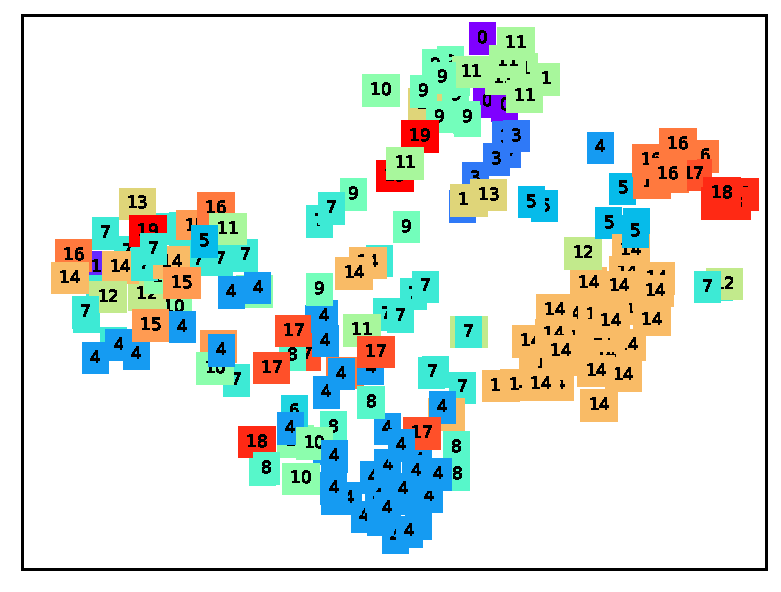
\includegraphics[width=.6\textwidth]{figs/visualization.pdf}
    \caption{t-SNE可视化分析结果}
    \label{fig:visualization}
\end{figure}
